% options:
% thesis=B bachelor's thesis
% thesis=M master's thesis
% czech thesis in Czech language
% slovak thesis in Slovak language
% english thesis in English language
% hidelinks remove colour boxes around hyperlinks

\documentclass[thesis=B,czech]{FITthesis}[2012/06/26]

\usepackage[utf8]{inputenc} % LaTeX source encoded as UTF-8

\usepackage{graphicx} %graphics files inclusion
\graphicspath{ {images/} }

\usepackage{listings}


% \usepackage{amsmath} %advanced maths
% \usepackage{amssymb} %additional math symbols

\usepackage{indentfirst}

\usepackage{dirtree} %directory tree visualisation

% % list of acronyms
% \usepackage[acronym,nonumberlist,toc,numberedsection=autolabel]{glossaries}
% \iflanguage{czech}{\renewcommand*{\acronymname}{Seznam pou{\v z}it{\' y}ch zkratek}}{}
% \makeglossaries

\newcommand{\tg}{\mathop{\mathrm{tg}}} %cesky tangens
\newcommand{\cotg}{\mathop{\mathrm{cotg}}} %cesky cotangens

% % % % % % % % % % % % % % % % % % % % % % % % % % % % % %
% ODTUD DAL VSE ZMENTE
% % % % % % % % % % % % % % % % % % % % % % % % % % % % % %

\department{Katedra \ldots (DOPLŇTE)}
\title{Doplňte název práce}
\authorGN{Tomáš} %(křestní) jméno (jména) autora
\authorFN{Šimáček} %příjmení autora
\authorWithDegrees{Tomáš Šimáček} %jméno autora včetně současných akademických titulů
\supervisor{Ing. Zdeněk Muzikář, CSc.}
\acknowledgements{Doplňte, máte-li komu a za co děkovat. V~opačném případě úplně odstraňte tento příkaz.}
\abstractCS{V~několika větách shrňte obsah a přínos této práce v~češtině. Po přečtení abstraktu by se čtenář měl mít čtenář dost informací pro rozhodnutí, zda chce Vaši práci číst.}
\abstractEN{Sem doplňte ekvivalent abstraktu Vaší práce v~angličtině.}
\placeForDeclarationOfAuthenticity{V~Praze}
\declarationOfAuthenticityOption{4} %volba Prohlášení (číslo 1-6)
\keywordsCS{Nahraďte seznamem klíčových slov v češtině oddělených čárkou.}
\keywordsEN{Nahraďte seznamem klíčových slov v angličtině oddělených čárkou.}

\begin{document}

% \newacronym{CVUT}{{\v C}VUT}{{\v C}esk{\' e} vysok{\' e} u{\v c}en{\' i} technick{\' e} v Praze}
% \newacronym{FIT}{FIT}{Fakulta informa{\v c}n{\' i}ch technologi{\' i}}

\begin{introduction}
    \input{chapters/Úvod.tex}
\end{introduction}

\chapter{Cíle práce}
    \input{chapters/Cíle.tex}

\chapter{Souborové systémy}
    V této kapitole je uvedena definice souborového systému a také jsou zde představeni nejznámější zástupci. V závěru této kapitoly vybrané zástupce porovnáme v několika ohledech.
\section{Souborový systém}
    \label{fs}
    Souborový systém označuje způsob, kterým se organizují data v datových úložištích. Jak už název napovídá, data jsou v úložišti organizována do souborů. <CITATE Soubor>
    Tento systém si o každém souboru udržuje informace, aby bylo později možné zjistit, kde se soubor nachází, jak je velký popřípadě jak se jmenuje. Dále tento systém umožnuje tyto data číst, měnit nebo vytvářet.

    V dnešní době existuje mnoho způsobů organizace dat, a proto máme k dispozici i mnoho různých souborových systémů. Ty se liší nejenom ve způsobu jak data organizují,
    ale také v možnostech jak velké datové úložiště dokáží adresovat nebo jak velké soubory dokáží spravovat. Další rozlišovacím prvkem může být závislost na operačním systémů.
    Jelikož nejrozšířenější operační systémy jsou systémy typu Unix a Windows, uvedeme několik typických zástupců souborových systémů pro tyto platformy.

    Mezi nejznámější zástupce unixových souborových systémů patří následující systémy.
    \begin{itemize}
      \item UFS
      \item ext2, ext3, ext4
    \end{itemize}

    Naopak mezi nejznámější zástupce pro platformu Windows se řadí navazující systémy.
    \begin{itemize}
      \item FAT12, FAT16, FAT32
      \item NTFS
    \end{itemize}

\section{Porovnání}
    V tabulce \ref{fscompare} můžeme vidět porovnání vybraných souborových systémů z hledska maximální délky názvu souboru, maximální velikosti souboru a maximální velikosti svazku, který dokáží spravovat.
    \begin{table}[]
    \centering
    \caption{Porovnání systémů souborů}
    \label{fscompare}
    \begin{tabular}{|l|l|l|l|}
    \hline
    Název & Max. délka názvu & Max. velikost souboru & Max. velikost svazku \\ \hline
    TODO & TODO & TODO & TODO \\ \hline
    \end{tabular}
    \end{table} 

\chapter{ZFS}
    Úvod následující kapitoly stručně popisuje vznik a historii souborového sytému ZFS. Zbytek této kapitoly představuje strukturu ZFS, jeho základní stavební kameny a některé zajímavé principy, které tento souborový systém využívá. Pro názornost jsou v této kapitole uvedeny praktické ukázky příkazů sloužící k administraci ZFS.

\section{Úvod}
    %NICM MOC
    Souborový systém Zettabyte byl původně vyvinut společností Sun Microsystems a následně integrován do operačního systémů Solaris od stejnojmenné společnosti.
    Jak už to tak v dnešním světě bývá v roce 2010 společnost Oracle akvizicí společnosti Sun Microsystem získala operační systém Solaris a tím i vlastnictví ZFS \cite{suns}. V dnešní době tedy veškerý vývoj a podpora pro tyto systémy pochází právě od firmy Oracle \cite{guide}. Tyto dokumenty byly i hlavním zdrojem informací pro tuto bakalářskou práci.

    Systém byl původně navrhnut pro použití čistě v operační systém Solaris, s čímž se pojily i minimální požadavky pro provoz ZFS, které jsou představeny v následujícím seznamu \cite{requirements}.
    \begin{itemize}
      \item Architektura procesoru SPARC nebo x86
      \item Operační systém Solaris 10 6/06 nebo novější
      \item Minimální místo na disku 128 MB
      \item Minimální místo pro vytvoření poolu 64 MB
      \item Pro optimální výkon ZFS alespoň 1 GB operační paměti
    \end{itemize}

    Díky zveřejnění zdrojových kódů ZFS, došlo k adaptaci souborového systému i na jiné operační systémy než je Solaris. Hlavním příkladem jsou systémy s Linuxovým jádrem jako je například Debian, Fedora nebo CentOS.

\section{Struktura}
Většina tradičních souborových systémů se váže na jedno konkrétní zařízení. Aby bylo možné spojit se souborovým systémem více zařízení, byl zaveden takzvaný volume manager, který souborovému systému poskytoval iluzi, že se jedná o samostatné zařízení \cite{traditional}. Ve skutečnosti se pod touto vrstvou může skrývat více disků, které se tváří jako jeden. ZFS se v tomto směru vydalo svojí vlastní cestou a zařízení agreguje do takzvaných poolů, které slouží jako datový základ pro jednotlivé souborové systémy.
\begin{figure}[!h]
    \caption{Agregace zařízení do poolu}
    \label{agregation}
    \centering
    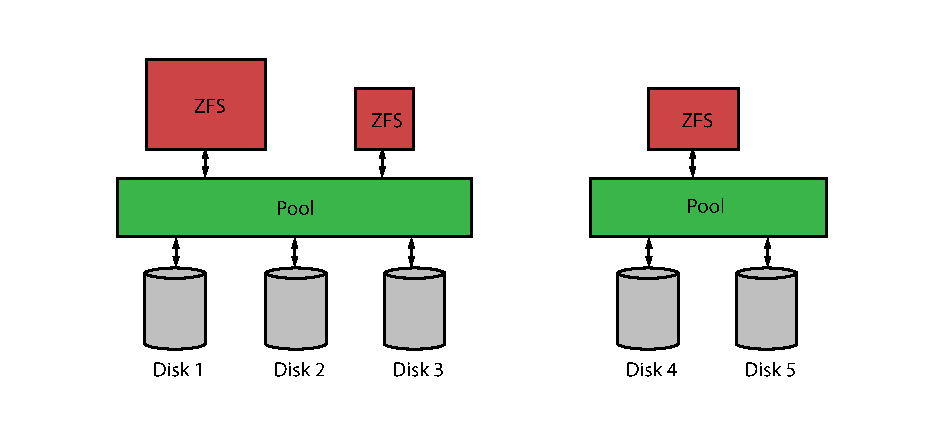
\includegraphics[scale=0.8]{agregation.pdf}
\end{figure}
\section{Pool}
Souborový systém ZFS se skládá ze dvou hlavních stavebních kamenů. Prvním z nich je takzvaný pool. V terminologii ZFS je to logické sdružení virtuálních zařízení, které popisuje rozložení a fyzické vlastnosti těchto zařízení \cite{terminology}. Pool je tedy spojení fyzických nebo virtuálních zařízení, které poskytuje základ pro souborové systémy ZFS.

Souborové systémy v ZFS se už neváží přímo na konkrétní fyzické zařízení, jak tomu bylo dříve, ale na pool jako celek. Historické spojení souborového systému s konkrétním fyzickým zařízením přinášela mnohá omezení. Například pokud jsme souborový systém chtěli rozšířit, museli jsme ho celý znovu vytvořit. Tato operace mohla být časově náročná, ale
v ZFS tomu tak není.
\subsection{Vlastnosti poolu}
ZFS si o každém vytvořeném poolu udržuje informace, které používá pro správu. Každý pool má seznam vlastností, které ho popisují a jednoznačně určují.
Hlavním identifikátorem poolu je jeho jméno. Toto jméno musí být v kontextu celého ZFS unikátní, protože se používá v příkazech manipulujících s daným poolem.

Vlastnosti můžeme rozdělit na dvě skupiny. Na jedné straně jsou statické vlastnosti, které popisují stav poolu a nedají se změnit přímo. Jsou takzvaně read-only. Pod tímto druhem vlastností si můžeme představit informace týkající se úložného prostoru jako je například velikost poolu, obsazená kapacita nebo volné místo. Velikost poolu nemůžeme změnit přímo nastavením odpovídající vlastnosti na jinou hodnotu, ale můžeme přidat do poolu další zdroj. ZFS tento krok rozpozná a související vlastnosti upraví.

Na druhé straně jsou vlastnosti, které můžeme měnit dynamicky. Některé z těchto vlastností se dají nastavovat pouze v okamžiku, kdy daný pool vytváříme nebo importujeme. Nastavit můžeme například vlastnost \emph{read-only}. Tato vlastnost zajistí, že od doby, kdy byla nastavena, lze z daného poolu data pouze číst a nikoliv data zapisovat. Další zajímavou vlastností je vlastnost \emph{bootfs}, která odkazuje na souborový systém uvnitř poolu, který slouží pro načítání operačního systému. Manuální nastavovaní této vlastnosti se nedoporučuje, protože špatné nastavení může vést k nenačtení operačního systému.

Následující příkaz umožňuje administrátorovi vypsat všechny vlastnosti daného poolu. Pro stručnost jsou vybrány pouze základní vlastnosti.
\begin{verbatim}
# zpool get all rpool
NAME   PROPERTY       VALUE                SOURCE
rpool  allocated      11.9G                -
rpool  bootfs         rpool/ROOT/solaris   local
rpool  capacity       38%                  -
rpool  dedupratio     1.19x                -
rpool  free           18.9G                -
rpool  health         ONLINE               -
rpool  readonly       off                  -
rpool  size           30.8G                -
\end{verbatim}

\subsection{Vytváření poolu}
Pool můžeme v systému ZFS kdykoli dynamicky vytvořit bez potřeby zásahu do operačního systému. Stačí když máme k dispozici potřebné zdroje (disk, partition, soubor) k vytvoření námi požadovaného poolu. Pokud máme požadované zdroje, stačí už jen vybrat unikátní jméno pro pool v kontextu ZFS a provést například následující příkaz.
\begin{verbatim}
$ zpool create tank c1t2d0 c2t1d0
\end{verbatim}
V případě dostupnosti disků c1t2d0 a c2t1d0, tento příkaz vytvoří pool jménem \verb|tank|đ, do kterého tyto disky přiřadí. Výsledná velikost bude součtem velikostí těchto disků. Takto vytvořený pool neobsahuje žádnou redundanci a v případě selhání disku, může dojít ke ztrátě dat. Druhým typem, které ZFS podporuje, jsou redundandní pooly.
\subsection{Zrcadlení}
Prvním druhem redundadních poolů jsou ty, které obsahují virtuální zařízení \emph{mirror} nebo-li zdcadlení. Tento typ virtuálního zařízení můžeme pomocí ZFS vytvořit nad dvěma a více zařízeními. Uvnitř zařízení dochází k replikaci dat na všechny disky v zařízení. Výsledná kapacita virtuálního zařízení je tedy rovna kapacitě jednoho disku. Pokud zrcadlení vytvoříme nad třemi disky, nakonec budou data na všech třech discích stejná a v případě výpadku dvou z nich o data nepřijdeme. Jiná situace je samozřejmě v případě výpadku všech tří disků najednou. Zrcadlení nám v tomto případě nepomůže a všechny data ztratíme. Nicméně pravděpodobnost, že dojde k výpadku všech tří disků najednou, než stihneme alespoň jeden vyměnit, je malá.

Následující příkaz demonstruje vytvoření poolu s redundantním zařízením \emph{mirror} o třech discích.
\begin{verbatim}
# zpool create Pool mirror c1t1d0 c1t2d0 c2t1d0
\end{verbatim}

\subsection{Raidz}
Druhým typem redundantních poolů, které ZFS umožňuje vytvářet, jsou pooly obsahující virtuální zařízení \emph{raidz}. Toto virtuální zařízení využívá jednoho nebo více paritních disků, které nám v případě výpadku nějakého disku umožní dopočítat ztracená data. Podle počtu paritních disků nám ZFS umožňuje vytvářet následující typy zařízení.
\begin{itemize}
  \item \emph{raidz1} - stripování s jedním paritním diskem
  \item \emph{raidz2} - stripování se dvěma paritními disky
  \item \emph{raidz3} - stripování se třemi paritními disky
\end{itemize}

Zápis dat na disk se provádí v pevně stanovených jednotkách tzv. stripech. Jeden stripe je rovnoměrně rozprostřen po všech datových discích virtuálního zařízení \emph{raidz}. Pokud bychom tedy zapisovali na disky soubor, který by měl přesně velikost stripu, soubor bude rovnoměrně rozprostřen na všech discích. Pokud by došlo k výpadku jednoho disku z virtuálního zařízení, dojde tím i k poškození určité části souboru a nebude možné tyto data přečíst. Pro tento účel se využívá paritních disků. Při zápisu stripu na disky se ze zapisovaných dat vypočte jedna hodnota, která se následně uloží na paritní disk. V případě výpadku jednoho disku z virtuálního zařízení, jsme schopni dopočítat chybějící data z hodnoty parity. Zvýšením počtu paritních disků jsme schopni dopočítat data při výpadku stejného počtu disků jako máme k dispozici paritních disků.
Pokud dojde v jednom okamžiku k výpadku více disků, než máme k dispozici paritních disků, dojde k nenávratné ztrátě dat.

Jelikož jsou data rovnoměrně rozmístěna na všechny disky ve virtuálním zařízení, můžeme při čtení dat využívat více disků najednou. Tím dokážeme docílit vyšší rychlosti čtení.

Následující příkaz ukazuje, jak jednoduše se dá v souborovém systému ZFS vytvořit redundantní pool typu \emph{raidz1}.
\begin{verbatim}
# zpool create Pool raidz1 c1t1d0 c1t2d0 c2t1d0 c2t2d0
\end{verbatim}

\subsection{Rozšiřování poolu}
Výhodou architektury poolů je možnost dynamického přidávání fyzických nebo virtuálních zařízení do poolu. Tím získáváme možnost dynamického rozšiřování kapacity celého poolu, která u tradičních souborových systému byla komplikovaná (nutnost použití VM) nebo nebyla dostupná vůbec. Souborové systémy v ZFS, které jsou vytvořené nad stejným poolem, sdílejí jeho prostředky, a proto při rozšiřování kapacity tohoto poolu budou mít k dispozici více místa pro ukládání dat.

V případě neredundantích poolů, které neobsahují virtuální zařízení typu \emph{mirror} nebo \emph{raidz}, můžeme pro rozšíření použít soubor, disk nebo část disku (partition). ZFS nám pro tento účel nabízí příkaz \verb|zfs add|, kterým můžeme dynamicky pool rozšiřovat.

Pokud pool obsahuje redundantní zařízení \emph{mirror} nebo \emph{raidz}, je doporučené pool rozšiřovat pouze o stejný typ zařízení. Pokud se do poolu typu \emph{mirror} pokusíme přidat virtuální zařízení \emph{raidz}, ZFS nás nám vypíše varovnou hlášku.

Využití souboru jako zdroje pro ZFS pool se v praxi téměř nevyužívá. Znamená to přidání další vrstvy mezi ZFS a samotný zdroj dat. Hlavní nevýhodou tohoto způsobu je značné zpomalení procesu čtení a zápisu dat, ale na druhou stranu se tato volba výborně hodí pro testování funkcí souborového systému ZFS.

\subsection{Zrušení poolu}
Stejně jako můžeme dynamicky pool vytvářet a rozšiřovat, můžeme pool i kdykoli zničit a uvolnit tak prostředky, které využíval. Tyto prostředky jsou ihned k dispozici a můžeme z nich vytvořit nový pool. Jelikož všechny souborové systémy vytvořené nad poolem sdílejí jeho prostředky, jsou tyto souborové systémy zničeny spolu s tímto poolem. Ke zničení poolu, který jsme dříve vytvořili, můžeme použít následující příkaz.
\begin{verbatim}
# zpool -r destroy tank
\end{verbatim}
Pokud v systému existuje pool jménem \verb|tank|, příkaz ho zničí bez ohledu na to, kolik souborových systému nad tímto poolem bylo vytvořeno.

\section{Souborový systém}
Druhým ze stavebních kamenů ZFS jsou samotné souborové systémy. Jak bylo zmíněno v kapitole \ref{fs}, souborový systém je způsob organizace dat do souborů v datových úložištích.
Tradiční souborové systémy využívají k organizaci různých datových struktur. Souborový UFS využívá tzv. inodů, což je datová struktura držící atributy souboru a ukazatele na jednotlivé datové bloky \cite{ufs}. Souborový systém FAT k organizaci dat využívá tzv. file allocation table \cite{fat}. ZFS k tomuto účelu využívá stromové datové struktury, která je znázorněna na obrázku \ref{structure}. Jedná se v podstatě o systém odkazů, který zároveň udržuje informace o souborech a adresářích. Bloky s daty se nacházejí v listech stromu.
\begin{figure}[!h]
    \caption{Struktura souborového systému ZFS}
    \label{structure}
    \centering
    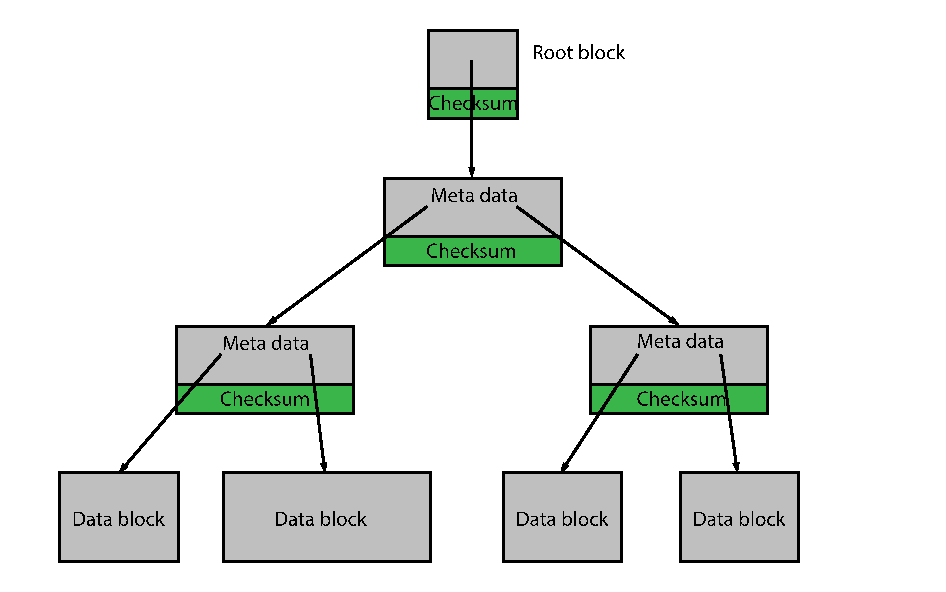
\includegraphics[scale=0.8]{zfsstructure.pdf}
\end{figure}

Tato stromová struktura přináší zajímavé výhody, které budou podrobněji popsány v dalších kapitolách.

\subsection{Hierarchie souborových systémů}
\label{hiararchy}
Jednou z vlastností ZFS je možnost hierarchického vnořování souborových systémů do sebe. Fakt, že samotný pool, jakožto zdroj místa pro souborové systémy, se chová jako samostatný souborový systém, tuto vlastnost dokazuje. Přesvědčit se o tom můžeme pomocí následujícího příkazu, kterému místo jména souborového systému předáme jméno poolu. Pokud příkaz proběhne dobře, vypíše základní informace o souborovém systému.
\begin{verbatim}
# zfs list rpool
NAME    USED  AVAIL  REFER  MOUNTPOINT
rpool  12.1G  18.2G  4.85M  /rpool
\end{verbatim}
Pokud by zmíněný souborový systém neexistoval, příkaz by vrátil chybovou hlášku.

Pool tedy tvoří hlavní uzel v této hierarchické posloupnosti a všechny souborové systémy vytvořené nad tímto poolem jsou jeho potomkem. V jednom poolu můžeme vytvořit více souborových systémů a také je do sebe můžeme libovolně vnořovat. Nejlépe si můžeme tuto hierarchii souborových systémů ukázat na obrázku \ref{fshierarchy}, kde můžeme vidět jak se do sebe jednotlivé souborové systémy vnořují.
\begin{figure}[h]
    \caption{Hierarchie souborových systémů ZFS}
    \label{fshierarchy}
    \centering
    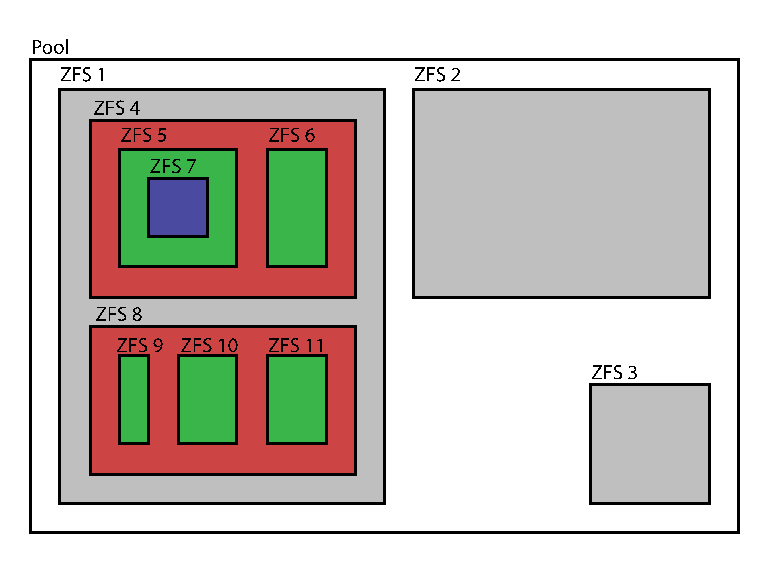
\includegraphics[scale=0.8]{hierarchy.pdf}
\end{figure}

\subsection{Vlastnosti souborového systému}
Stejně jako si ZFS udržuje u každého poolu jeho vlastnosti, udržuje si je také u každého souborového systému. Nastavováním těchto vlastností je administrátor schopen určit specifické chování konkrétního souborového systému. V kontextu ZFS má každý souborový systému jednoznačný identifikátor, který je odvozen z hierarchie souborových systémů. Skládá se z názvu systému a jeho rodičů. Identifikátor by mohl vypadat následovně \emph{rpool/ROOT/solaris}.

Vlastnosti souborových systémů můžeme rozdělit, stejně jako u vlastností poolu, na dvě kategorie. První kategorií jsou vlastnosti, které se dají pouze číst. Velkou část této skupiny tvoří vlastnosti popisující využití místa v souborovém systému. Příkladem může být místo spotřebované vnořenými souborovými systémy nebo souborovým systémem samotným. V této skupině vlastností můžeme najít také datum vytvoření nebo poměr deduplikace a komprese dat.

V druhé kategorii jsou vlastnosti, které může administrátor změnit za běhu nebo při vytváření souborových systémů. Stejně jako na úrovni poolu, tak i na úrovni souborového systému, můžeme nastavit vlastnost \emph{read-only}, která znemožní uživatelům zapisovat nebo měnit data v souborovém systému. Za povšimnutí dále stojí vlastnost \emph{exec}, která dovoluje v souborovém systému spouštět procesy.

Administrátor může jednoduše zapínat, vypínat či měnit vlastnosti souborového systému pomocí příkazu \verb|zfs set property=value rpool|, popřípadě si zobrazit seznam všech dostupných vlastností o souborovém systému pomocí \verb|zfs get all rpool|.

\subsection{Dědičnost}
Díky hierarchické struktuře se dá jednoduše zjistit, kdo je předkem daného souborového systému a kdo je jeho potomkem. Všechny nastavitelné vlastnosti, kromě kvót a rezervací, se dědí od rodičovského souborového systému. Pokud žádný rodič nemá vlastnost nastavenou explicitně, je použita standardní hodnota \cite{inheriting}.

Pokud chceme explicitně říci, aby některá vlastnost byla převzata od rodiče, můžeme použít příkaz \verb|zfs inherit property rpool|. Tento příkaz odnastaví danou vlastnost ze souborového systému a pokusí se převzít hodnotu z rodiče. Pokud v žádném z rodičů není hodnota nastavena explicitně, je použita standardní hodnota \cite{inheriting}.
\subsection{Vytváření souborového systému}
\label{createfs}
Vytváření souborových systémů v ZFS je velice jednoduché. Jediné co potřebujeme k vytovření souborového systému je jednoznačný identifikátor. ZFS umožnuje vytvoření těchto systémů pomocí příkazu \verb|zfs create pool|, kde \emph{pool} je indentifikátor. Pokud neexistují všichni předci, je potřeba použít přepínač \verb|-p|, jinak příkaz selže.

Při vytváření je možné specifikovat, které vlastnosti daný souborový systém bude mít. Mimo jiné existují vlastnosti, které se dají nastavit pouze při vytváření. Po vytvoření souborového systému jsou tyto vlastnosti vedeny jako read-only a nedají se změnit. Jako příklad můžeme uvést vlastnost \emph{encryption}, která umožňuje šifrování souborového systému pomocí různých kryptografických funkcí. Pro využití této vlastnosti můžeme při vytváření poolu použít následující přepínač následující příkaz.
\begin{verbatim}
# zfs create -o enryption=on tank/pool/pool
\end{verbatim}
\subsection{Zrušení souborového systému}
Rušení souborových systému je v ZFS stejně snadné jako jejich vytváření. Je důležité mít na paměti, že zrušením souborového systému, který má nějaké potomky, zrušíme i všechny vnořené souborové systémy. Pro zrušení souborového systému pak již stačí použít příkaz \verb|zfs destroy| s příslušným identifikátorem, popřípadě přepínačem \verb|-r| pro zrušení všech potomků.
\subsection{Kvóty}
\label{quota}

Kvóty v ZFS umožňují administrátorovi spravovat limity souborových systémů týkajících se využitého místa. Tyto limity omezují možnosti využití dostupného místa v souborovém systému. Kvóty můžeme rozdělit do následujících kategorií podle toho, koho omezují.
\begin{itemize}
  \item Obecné - týkající se souborového systému
  \item Uživatelské - omezují jednotlivé uživatele
  \item Skupinové - omezují celé skupiny uživatelů
\end{itemize}

Obecné kvóty omezují místo, které může souborový systém využít jako celek. K tomuto účelu v ZFS slouží vlastnost \emph{quota}, která stanovuje limit místa, které může daný souborový systém využít. V tomto případě se do využitého místa započítává i místo spotřebované potomky \cite{quotas}. Pokud bychom chtěli omezit souborový systém bez ohledu na to kolik místa využijí jeho potomci, musíme použít vlastnost \emph{refquota}.
%% Rezervace

Vzhledem k faktu, že souborové systémy v jednom poolu sdílí diskové místo, ZFS přichází s vlastností \emph{reservation}. Tato vlastnost oproti kvótám garantuje souborovému systému diskové místo dané velikosti \cite{quotas}. Stejně jako v případě vlastnosti \emph{quota} je toto místo vyhrazeno pro souborový systém a všechny jeho potomky. Pokud bychom chtěli garantovat místo přímo souborovému systému, bez ohledu na to kolik místa využívají jeho potomci, musíme využít vlastnost \emph{refreservation}.

Jelikož vlastnosti \emph{quota} resp. \emph{refquota} a vlastnosti \emph{reservation} resp. \emph{refreservation} jsou vlastnostmi souborového systému, můžeme je nastavit stejně jako kteroukoliv jinou vlastnost pomocí následujících příkazů.
\begin{verbatim}
# zfs set quota=10G rpool/export/home
# zfs set reservation=10G rpool/export/home
\end{verbatim}

Vztahy mezi vlastnostmi \emph{quota} a \emph{reservation} jsou vyznačeny na obrázku \ref{quotavsreserv}.
%% Obrázek
\begin{figure}[h]
    \caption{Vztahy mezi vlastnostmi \emph{quota} a \emph{reservation}}
    \label{quotavsreserv}
    \centering
    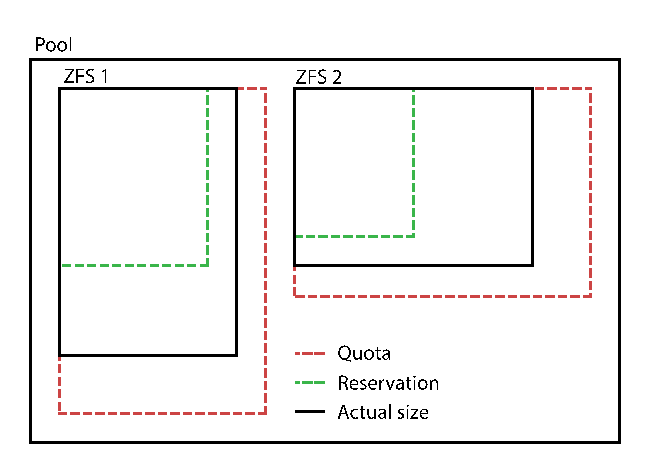
\includegraphics[scale=0.8]{quota.pdf}
\end{figure}
%% Uživatelské a skupinové kvóty

Další možností, jak omezit využití diskového místa, je pomocí uživatelských resp. skupinových kvót. Tyto kvóty limitují uživatele resp. skupinu v tom, kolik místa můžou v souborovém systému využít. Každý souborový systém má svůj vlastní \emph{userspace} resp. \emph{groupspace}, kde si udržuje informace o tom jaké mají limity jednotlivé skupiny resp. uživatelé.
Administrátor si může hodnoty uživatelských resp. skupinových kvót vypsat pomocí \verb|zfs userspace| resp. \verb|zfs groupspace|. Následující příkaz demonstruje, jak vypadá výpis uživatelských kvót pro domovský adresář.
\begin{verbatim}
# zfs userspace rpool/export/home/simactom
TYPE        NAME       USED  QUOTA  SOURCE
POSIX User  root      1.50K   none  default
POSIX User  simactom   641M   none  default
\end{verbatim}

Pokud se uživatel resp. skupina v seznamu nenachází nebo je u něj uvedena hodnota \emph{none}, uživatelské resp. skupinové kvóty se na něj nevztahují. Je-li v seznamu uvedena jiná hodnota, pak uživatel v daném souborovém systému nesmí překročit tuto hodnotu. Pokud by tuto hodnotu překročil, systém ho varuje a požadovanou akci neprovede. Přiřazení kvóty uživateli resp. skupině provedeme pomocí následujících příkazů
\begin{verbatim}
# zfs userquota@username=value filesystem
# zfs groupquota@username=value filesystem
\end{verbatim}

ZFS nabízí ještě vlastnost \emph{defaultuserquota} resp. \emph{defaultgroupquota}, kterou lze nastavit na určitou hodnotu. Tento limit se použije v případě, že hodnotu uživatelské resp. skupinové kvóty nastavíme na \emph{default}.
\section{Deduplikace}
\label{dedup}
Jednou z další vlastností, které ZFS nabízí, je deduplikace. Jak již z názvu vyplývá, jedná se o proces, který zabraňuje duplikaci stejných dat na disku a tím šetří i místo. Deduplikace se obecně dá rozdělit na následující úrovně.
\begin{itemize}
  \item Úroveň souborů
  \item Úroveň datavých bloků
  \item Úroveň bajtů
\end{itemize}

K identifikaci stejných dat se v ZFS využívá hešovácí funkce. Z porovnávaných dat jsou vytvořeny heše, které jsou následně porovnány. Pokud se heše rovnají a používáme kvalitní hešovací funkci, můžeme s velkou pravděpodobností říci, že jsou porovnávaná data opravdu totožná \cite{dedup}. Pokud je administrátor z nějakého důvodu stále nedůvěřivý, může u vlastnosti deduplikace nastavit hodnotu \emph{verify}, která zajistí celkové porovnání datových částí bajt po bajtu.

Deduplikace na úrovni souborů využívá nejméně systémových prostředků, protože se data hešují a porovnávají po velký částech. Na druhou stranu sebemenší změna v souboru vyžaduje přepočítání heše, který se již bude lišit od původního \cite{dedup}. Souborový systém pak rozpozná, že se soubory liší a uspořené místo bude zaplněno změněným souborem.

Deduplikace datových bloků vyžaduje oproti deduplikaci souborů vyšší využití systémových prostředků, ale na druhou stranu přináší v jistých situacích lepší úsporu místa \cite{dedup}.

V poslední řadě existuje deduplikace na úrovni bajtů, která je ze všech uvedených úrovní nejnáročnější na využití výpočetních prostředků. Tato možnost se používá jen ve speciálních případech.

ZFS z výše uvedených možností nabízí právě deduplikaci na úrovni datových bloků, protože tato jednotka deduplikace přináší nejvíce výhod v obecných případech použití \cite{dedup}. Na obrázku \ref{blockdedup} můžeme vidět porovnání souborového systému při zapnuté a vypnuté vlastnosti deduplikace.
\begin{figure}[!h]
    \caption{Ukázka deduplikce na úrovni datový bloků}
    \label{blockdedup}
    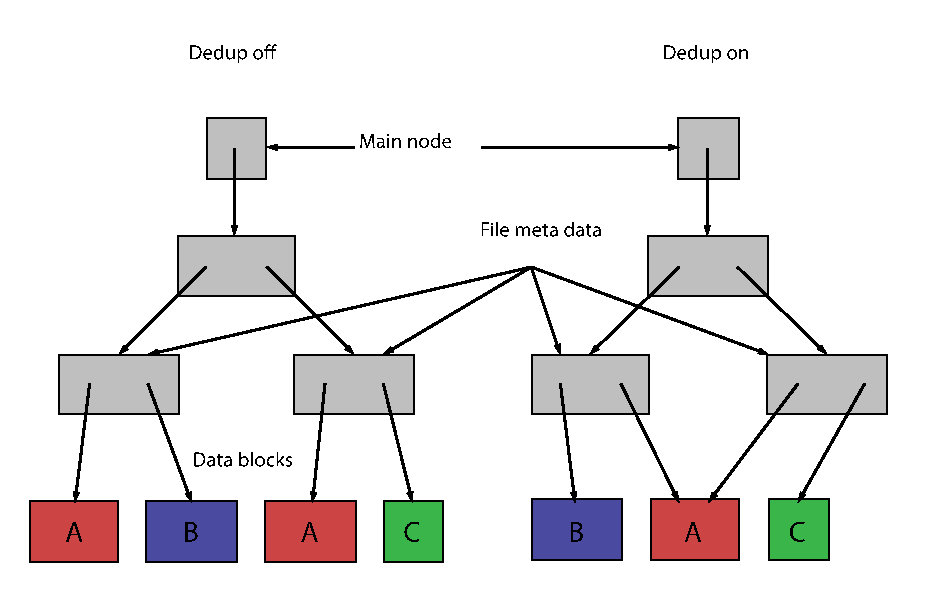
\includegraphics[scale=0.8]{dedup.pdf}
\end{figure}
\section{Konzistence}
\label{consitence}
Starší souborové systémy zapisují data přímo do bloku, který mění. To může v některých případech, jako je selhání systému nebo výpadek proudu, vést k nekonzistenci souborového systémů. V takovém případě je nutné celý souborový systém zkontrolovat například pomocí příkazu \verb|fsck|. Bohužel ani tento nástroj v některých případech nedokáže některé nekonzistence opravit \cite{transaction}.

Některé souborové systémy využívají tzv. žurnálů k pomoci s udržování konzistence dat. Žurnál je speciální záznam, kam se ukládají informace o tom, co a kde se bude měnit. Po provedení popisované akce se do žurnálu zapíše, že daná operace byla provedena. Když systém zkolabuje v jakémkoli kroku tohoto postupu, je možné ho při startu sytému dostat do konzistentního stavu. K tomuto účelu se opět využívá nástroj \verb|fsck|.

ZFS přichází s transakčním systémem a technikou copy on write. Tato technika zajišťuje neustálou konzistenci souborového systému i v okamžiku výpadku, a proto není třeba žurnálu. Data na disku nejsou nikdy přímo přepisována \cite{transaction}.

Transakce může vypadat následovně. Nejprve se vytvoří kopie bloků, které mají být změněny. V těchto kopiích dojde k vlastní změně dat, zatímco původní data jsou stále na disku a nejsou nijak změněna. Následně se provede kopie potřebných metadat, které se týkají měněných datových bloků. Tyto metadata jsou následně přepočítána podle nových datových bloků a konečně v poslední řadě se provede atomická operace, která připojí větev s novými resp. změněnými bloky do stromu souborového systémů. Stará data jsou smazána.

Průběh transakce je naznačen na obrázku \ref{cow}. Celá transakce buď proběhne v pořádku nebo nebude přijata vůbec. Pokud v průběhu transakce dojde k výpadku, celý souborový systém zůstává konzistentní, protože původní data jsou stále na disku a nemohla se provést atomická operace, která by připojila nové data.
\begin{figure}[h]
    \caption{Demostrace copy on write}
    \label{cow}
    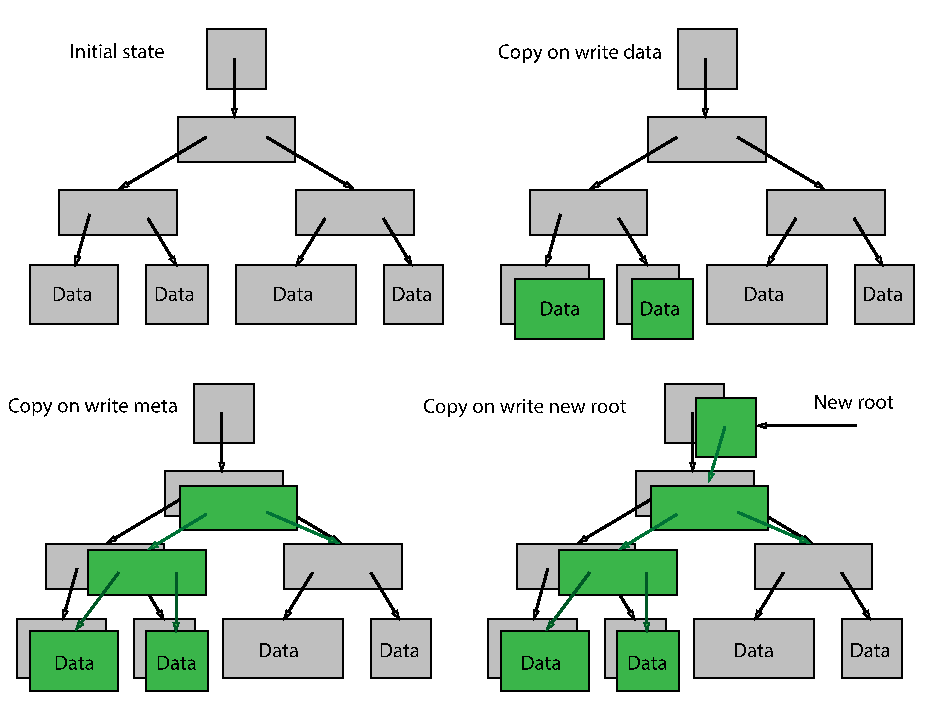
\includegraphics[scale=0.8]{cow.pdf}
\end{figure}
\section{Integrita dat}
\label{checksum}
Od souborového systému očekáváme, že při čtení dat z určitého datového bloku z disku, dostaneme data, která do tohoto bloku byla dříve zapsána. Pokud tomu tak není, měl by to souborový systém detekovat a vrátit chybu \cite{integrity1}.

Vlastnost neustálé konzistence souborového systému ZFS, zmíněná výše v kapitole \ref{consitence}, zajišťuje, že chybná data se v souborovém systému mohou vyskytnout jen chybou hardwaru \cite{integrity2}.

ZFS dokáže tyto chyby detekovat pomocí tzv. kontrolních součtů. Tyto součty vznikají a jsou přepočítávány při každé změně bloku v souborovém sytému. Jak jsme mohli vidět na obrázku \ref{structure}, součty nejsou uloženy v bloku, kterého se týkají, ale v bloku jemu nadřazeném. Při každém požadavku na čtení dojde k vypočítání kontrolního součtu na základě dat, které se v souborovém systému momentálně nachází a poté dojde k porovnání vypočteného součtu se součtem uloženým v nadřazeném bloku \cite{integrity1}. Tím ZFS dokáže rozhodnout zda je blok poškozený či nikoliv.

Díky těmto kontrolním součtům se souborový systém dokáže v určitých situacích sám opravovat. Tato situace nastává v případě, že blok, při jehož čtení došlo k chybě, je součástí redundantího virtuálního zařízení \emph{raidz} nebo \emph{mirror}. V tomto případě ZFS přečte datový blok i z replikovaného disku popřípadě sestaví blok pomocí parity a následně opraví chybný blok, při jehož čtení došlo k chybě. Aplikace dostane správná data i přes to, původně načtený datový blok byl poškozený.

Ačkoliv dochází k ověřování integrity dat automaticky při každém čtení z disku, je možné tento proces manuálně vyvolat a ověřit pomocí následující sekvence příkazů.
\begin{verbatim}
# zpool scrub pool
# zpool status pool
pool: pool
state: ONLINE
scan: scrub repaired 0 in 6s with 0 errors
\end{verbatim}

\section{Mountpoint}
\label{mountpoint}
Mounpoint je jednou ze základních vlastností všech souborových systémů. Je to vlastně cesta k bodu v adresářovém stromu operačního systému, kde má být daný souborový systém připojen.

Jelikož se ZFS snaží administrátorům maximálně ulehčit práci, stará se o automatické připojování souborových systémů sám. K účelům připojování souborových systémů v ZFS slouží jejich vlastnost \emph{mountpoint}, kde administrátor může specifikovat, kam se má daný souborový systém připojit. Pokud administrátor tuto vlastnost explicitně neurčí, je odvozena od vlastnosti rodičovského souborového systému.

Pro připojování souborových systémů ZFS se dají použít i tradiční nástroje \emph{mount} a \emph{umount}. V tradičních souborových systémech se pro automatické připojování používal soubor \emph{/etc/vsfstab}, kde administrátor specifikoval co a kam se má připojit. Operační systém po svém startu tento soubor zpracoval a vyznačené souborové systémy automaticky připojil.

Jak již bylo zmíněno, ZFS proces automatického připojování provádí samo. Pokud by administrátor chtěl využívat tradičního připojování pomocí souboru \emph{/etc/vsfstab}, je možné nastavit vlastnost \emph{mountpoint} souborového systému na hodnotu \emph{legacy} \cite{mountpoint}. Tím administrátor řekne, že se o souborový systému bude starat sám a ZFS ho již automaticky připojovat nebude.
\section{Snapshot}
\label{snapshot}
ZFS snapshot je stav daného souborového systému v čase, kdy byl snapshot pořízen. Jedná se read-only instanci daného souborového systému \cite{snapshot}.

Díky stromové architektuře souborového systému ZFS je pořizování snapshotů velice elegantní a nenáročné. Pro vytvoření můžeme použít příkaz \verb|zfs snapshot filesystem@snapshot|, kde \emph{filesystem} je jméno souborového systémů, jehož stav chceme zachytit a \emph{snapshot} je pojmenování konkrétního stavu tohoto systému.

Po provedení příkazu si ZFS zapamatuje odkaz na vrchol souborového systému, jehož snapshot tvoříme. Tento odkaz se stane hlavním kořenem snapshotu jakožto nového souborového systému. Jelikož snapshot je souborový systém určený pouze ke čtení, nemůžeme pomocí něj změnit data v aktivním souborovém systému. Po vytvoření snapshotu je jeho velikost nulová, protože se provedlo pouze zapamatování odkazu a nebyly vytvořeny žádné kopie. Pokud se ovšem data v aktivním souborovém systému změní, je nutné, aby snapshot stále odkazoval na stará data. Toho docílíme tak, že stará data zkopírujeme a zvětšíme tak velikost snapshotu \cite{snapshot}. Rozšiřování velikosti snapshotu tedy závisí na množství změněných dat od chvíle, kdy byl snapshot vytvořen. Proces vytváření snapshotu a rozšiřování jeho velikosti je názorně ukázán na obrázku \ref{snapshotproces}.
\begin{figure}[h]
    \caption{Vytváření snapshotu}
    \label{snapshotproces}
    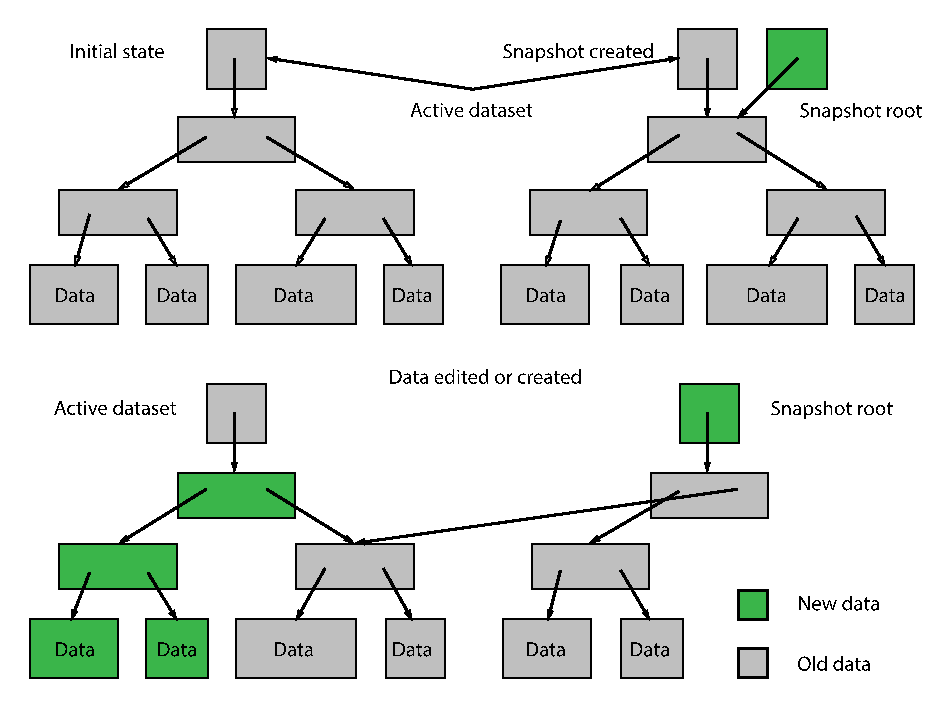
\includegraphics[scale=0.8]{snapshot.pdf}
\end{figure}

Rekurzivní tvorba snapshotů se provádí rychle pomocí jedné atomické operace. Snapshoty jsou vytvořeny naráz všechny dohromady nebo nejsou vytvořeny vůbec. Výhodou atomické operace je fakt, že data ve všech snapshotech jsou konzistentní vzhledem k jednomu časovému okamžiku \cite{snapshot}.

Snapshot pro souborový systém a všechny jeho potomky můžeme vytvořit pomocí následujícího příkazu.
\begin{verbatim}
# zfs snapshot -r rpool/export/home@snap
# zfs list -t snapshot -r rpool/export/home
NAME                             USED  AVAIL  REFER  MOUNTPOINT
rpool/export/home@snap              0      -    33K  -
rpool/export/home/simactom@snap     0      -   641M  -
\end{verbatim}
Druhý příkaz v pořadí ukazuje skutečnost, že snapshoty byly opravdu vytvořeny i pro všechny potomky daného souborového systému a že jejich velikost je opravdu nulová.

Snapshot se dá použít k navrácení souborového systému do stavu, v jakém se nacházel v okamžiku vytvoření snapshotu. Veškeré změny, které proběhly v souborovém systému od okamžiku vytvoření snapshotu budou smazány. K vyvolání tohoto procesu stačí použít příkaz \verb|zfs rollback snapshot |, kde \emph{snapshot} je celé jméno snapshotu. Jelikož se každý snapshot váže přímo s určitým souborovým systémem, není třeba zadávat jméno souborového systému, který chceme navrátit do původního stavu. 
    
\chapter{Analýza implementovaných řešení}
    V následující kapitole jsem si vybral několik nástrojů sloužící pro monitorování a správu souborového systému ZFS, které jsem zkoumal. Hlavně jsem se snažil najít výhody a nevýhody, které by mi mohli pomoci správně navrhnout vlastní řešení administračního nástroje pro ZFS.
\section{zfsmon}
Hlavním nástrojem, který jsem podrobil analýze, je \emph{Zfsmon}. Tento nástroj slouží pro monitorování souborových systémů ZFS na více oddělených souborových serverch. Aplikace má dvě oddělené části.

První částí je skript, který běží na počítači se souborovým systémem ZFS. Tento skript je spouštěn pomocí \emph{crontabu} a zajišťuje aktualizaci informací v databázi, která je součástí webové aplikace. \emph{Crontab} je program, který zajišťuje automatické spouštění skriptů v systému v určitých intervalech. Doporučený interval spouštění scriptu je 15 minut.<CITATE Zfsmon>

Druhou částí aplikace \emph{zfsmon} je samotná webová aplikace, která se stará o zobrazování dat z databáze. V databázi se nacházejí informace o stavu jednotlivých souborových systémů z různých serverů. Aplikace zobrazuje tyto informace zobrazuje klientovi v podobě HTML stránek.

Velkou výhodou této aplikace je, že dokáže zobrazovat informace z více oddělených úložišť najednou. Nadruhou stranu způsob zpracování dat přináší značnou nevýhodu, která spočívá v intervalu aktualizace dat v databázi. V průběhu tohoto intervalu aplikace znemožňuje uživateli vidět aktuální data ze ZFS úložiště. Uživatel je nucen počkat na konec tohoto intervalu, kdy jsou opět nahrána aktuální data do databáze. Další nevýhodou toho nástroje je absence veškeré funkcionality, která by s týkala administrace souborového systému ZFS.

Tento nástroj nám tedy umožňuje kvalitně monitorovat informace z více zdrojů najednou, ale neposkytuje nám možnost jakékoli administrace minitorovaných souborových systémů.
\section{zfswatcher}
Druhým nástrojem, který jsem si vybral k popisu je nástroj jménem \emph{Zfswatcher}.

Tento nástroj slouží jako webové rozhraní pro sledování souborového systému ZFS. Stejně jako předchozí nástroj zpracovává periodicky data a zobrazuje je pomocí HTML stránek, s čímž souvisí stejný problém, který jsem popsal u předchozího nástroje. Oproti nástroji \emph{Zfsmon} umí zobrazovat informace pouze z jednoho souborového serveru. Nadruhou stranu tento nástroj umí, v případě změny stavu, ZFS poslat upozornění v podobě e-mailu nebo zalogování do logu.<CITATE zfswatcher>
\section{ZFS administration console}
Na závěr této kapitoly bych chtěl jen zmínit nástroj \emph{smcwebserver}. Tento nástroj je součástí operačního systému Solaris 10 6/06 a umožňuje administrátorovi spravovat některé funkce tohoto operačního systému. Mimo jiné se část tohoto nástroje věnuje právě správě souborového systému ZFS.<CITATE smc> Bohužel v novější verzi Solarisu 11 se tento nástroj již nevyskytuje. Ze zmíněných nástrojů právě \emph{smcwebserver} nabízí administrátorovi i funkce pro administraci.

\chapter{Návrh řešení}
    \input{chapters/Návrh.tex}
\chapter{Implementace}
    Obsahem následující kapitoly popis vlastní implementace nástroje pro správu ZFS. Dále tato kapitola obsahuje postup, jak vytvořený nástroj integrovat do operačního systému Solaris.
\section{Python}
Než začneme s implementací, je nutné si ujasnit v jakém jazyce budeme aplikaci psát.

V operační systému Solaris příkazovou řádku interpretuje \emph{shell}, který nám dovoluje využívat funkce tohoto operačního systému. Jak jsem zmínil v minulých kapitolách, ZFS je součástí Solarisu a \emph{shell} nám dovoluje využívat jeho rozhraní, které je dostupné právě z příkazové řádky. Z počátku se tedy možnost skriptování v \emph{shellu} zdála jako dobrá volba. Nicméně \emph{shell} nám nedovoluje využívat výhody objektového programování, protože nepodporuje třídy. To je v rozporu s naším návrhem, který využívá objektové architektury MVC.

Z výše uvedeného důvodu jsem se rozhodl pro volbu skriptovacího jazyka \emph{python 2.7}, který nám umožní implementaci objektově orientované architektury MVC. Další výhodou tohoto jazyka je jeho přenositelnost. Interpret \emph.{pythonu} totiž existuje pro nejrůznější operační systému jako je Linux, Windows a samozřejmě náš Solaris. Tento fakt nám v konečném důsledku nebude moc užitečný, protože ZFS je dostupné primárně jen pro Solaris a implementace našeho nástroje se bude ubírat právě tímto směrem.
\section{HTTP Server}
Při návrhu aplikace jsme zvolili webové rozhraní. Pro implementaci tohoto řešení budeme muset zvolit nějaký webový server, který nám bude zprostředkovávát komunikaci mezi naší aplikací a webovým klientem (prohlížečem). Od našeho webového serveru budeme požadovat podporu HTTPS protokolu, tedy šifrování přenosu dat a možnost autentizace uživatelů pomocí metody \emph{Basic} protokolu HTTP.
    \subsection{Implementované řešení}
    Jednou z možností je vybrat si z velkého množství webových serverů, které jsou již implementované. Mezi nejznámější a nejrozšířenější zástupce patří například \emph{Apache}. Tato komplexní implementace webového serveru by jistě dokázala splnit všechny naše požadavky, ale přinesla by s sebou jistě i mnoho funkcí, které by naše aplikace vůbec nevyužila. Nehledě na to, by byl administrátor nucen tento webový server nainstalovat a správně nakonfigurovat, aby odpovídal požadavkům aplikace. Z tohoto důvodu jsem se rozhodl zvolit vlastní řešení webového serveru, které bude přesně odpovídat požadavkům aplikace.
    \subsection{Vlastní řešení webového serveru}
    Implementace vlastního řešení webového serveru bude využívat dvou standardních knihoven jazyka \emph{python} a bude se skládat z následujícíh tříd.
    \begin{itemize}
      \item \verb|WzfsadmServer|
      \item \verb|WzfsadmRequestHandler|
      \item \verb|Authenticator|
    \end{itemize}

    Tyto třídy dohromady budou tvořit webový server, který bude zprostředkovávat komunikaci mezi logickou částí aplikace a webovým prohlížečem. Součástí těchto tříd bude i implementace navržených bezpečnostních opatření.
    \subsubsection{Třída WzfsadmServer}
    Jelikož HTTP je textový protokol, použijeme jako základ celého serveru  třídu \verb|TCPServer|, která zajistí funkcionalitu TCP serveru a třídu \verb|ThreadingMixIn| zajišťující zpracování více požadavků v jednom okamžiku. Obě tyto třídy jsou součástí knihovny \verb|SocketServer|<CITATE SocketServer>, která je standardní součástí jazyka \emph{python}.

    Třída \verb|WzfsadmServer| reprezentující vlastní webový server, bude potomkem tříd \verb|TCPServer| a \verb|ThreadingMixIn| abychom dosáhli požadované funkcionality. To znamená, že zdědí metody obou rodičovských tříd a bude tyto metody moci využívat. Některé zděděné metody budeme nuceni přepsat pro dosažení zabezpečení přenosu dat.

    Hlavním úkolem této třídy je poslouchat příchozí spojení na předem stanoveném síťovém rozhraní a portu. Tyto informace budou předány instanci této třídy při jejím vytváření. Při vytváření instance dojde k vytvoření hlavního socketu, který následně propojíme se stanovenou IP adresou a síťovým portem. Dále server jen vyčkává do, okmažiku kdy se klient pokusí připojit. V tomto okamžiku, je vytvořen nový socket, který bude sloužit pro výměnu dat mezi klientem a serverem. Na této úrovni jsme schopni filtrovat IP adresy, které se k serveru budou moci připojovat. V konfiguračním souboru serveru budeme schopni napříkald stanovit, že se serverem lze komunikovat pouze z lokálního počítače.

    Pro samotnou výměnu dat mezi serverem a klientem, použijeme specializovanou třídu \verb|WzfsadmRequestHandler|, která bude umět komunikovat pomocí HTTP protkolu. Při každém připojení klienta k serveru vytvoříme instanci této třídy a předáme ji odkaz na spojení, kde bude docházet k výměně dat. Tato instance pak danný HTTP požadavek dokáže díky své implementaci vyřešit.

    Jelikož chceme šifrovanou komunikace, musíme už při vytváření instance třídy \verb|WzfsadmRequestHandler| předat odkaz na šifrované spojení. Pro tento účel budeme muset přepsat metodu \verb|get_request()| knihovní třídy \verb|TCPServer|. Tato metoda vrací odkaz na spojení, které umožňuje přenos dat a které předáváme třídě \verb|WzfsadmRequestHandler|. Aby tato metoda vracela odkaz na šifrované spojení, použijeme knihovnu \verb|ssl| a její funkci \verb|wrap_socket()|, která původní spojení začne šifrovat pomocí stanovené šifrovací metody.

    Aby bylo možné využít šifrování pomocí knihovny \verb|ssl|, budeme muset vytvořit privátní klíč pro šifrování a certifikát, kterým se server bude identifikovat. Tuto dvojici můžeme vytvořit například pomocí nástroje \verb|openssl|. Cestu k souborům s klíčem a certifikátem pak předáme funkci \verb|wrap_socket()| při jejím volání.

    Ke spuštění serveru stačí vytvořit instanci třídy \verb|WzfsadmServer| s požadovanými parametry a následně na této instanci zavolat metodu \verb|serve_forever()|. Od této chvíle bude server naslouchat na stanovené adrese a portu dokud nebude ukončen.


    \subsubsection{Třída WzfsadmRequestHandler}
    Další součástí webového serveru je již zmíněná třída \verb|WzfsadmRequestHandler|, která bude zajišťovat vlastní komunikaci s klientem pomocí HTTP protokolu. Při vytváření jí předáváme odkaz na šifrované připojení, tudíž veškerá komunikace bude zabezpečená pomocí HTTPS protokolu. Tato třída je potomkem třídy \verb|BaseHTTPRequestHandler|, která je součástí standardní knihovny \verb|BaseHTTPServer|. Tuto třídu si opět budeme muset přízpůsobit, protože v základu nepodporuje metodu \emph{Basic} protokolu HTTP, kterou chceme používat pro autentizaci uživatelů.

    Úprava bude vcelku jednoduchá. Do metody, která zpracovává jednotlivé požadavky, přidáme volání funkce, která ověří, zda-li klient poslal autentizační údaje. Poznáme to tak, že v hlavičkách požadavku HTTP protokolu bude obsažena hlavička \emph{Authorization}. Pokud klient tyto údaje nepošle, odpovíme na požadavek HTTP kódem 401 (Unauthorize). Jestliže údaje v hlavičkách najdeme pokusíme se uživatele ověřit. K tomuto účelu vytvoříme instaci třídy \verb|Authenticator| a na ní zavoláme metodu \verb|authenticate()|, které ověřované údaje předáme. Metoda nám pak vrátí zprávu, zda uživatel  byl či nebyl autentizován. Pokud metoda vrátí úspěch, uživatel je autentizován a je mu povolen vstup do aplikace. Jestliže metoda vrátí neúspěch, je odeslán kód 401 (Unauthorize).

    Pokud chceme metodou \emph{Basic} chránit celou aplikaci, musíme do hlaviček každé HTTP odpovědi zahrnout hlavičku \emph{WWW-Authenticate} jejíž hodnotou bude \emph{Basic}. Tím dáme webovému prohlížeči na straně klienta najevo, že vyžadujeme autentizaci uživatelů.

    V dalším kroku se v případě správné autentizace uživatele zavolá požadovaná HTTP metoda. Jelikož pro naše účely naší aplikace budou stačit prostředky, které nabízí metoda GET, ostatní metody nebude náš webový server podporovat. V případě, že klient pošle požadavek na jinou HTTP metodu než je GET, server odpoví kódem 501 (Not Implemented). Uvnitř metody, která reprezentuje HTTP metodu GET, server ověří, zda požadovaná URL odpovídá souboru. Server bude tento soubor hledat v kořenovém adresáři, který mu nastavíme pomocí konfiguračního souboru. Pokud URL odpovídá nějakému souboru, je jeho obsah odeslán klientovi a volání metody ukončeno. V opačném případě server vytvoří instanci třídy \verb|App| reprezentující naší aplikaci. Následně na této instanci zavolá metodu \verb|route|, které předá URL požadovanou klientem. Aplikace požadavek zpracuje a server v konečné fázi odešle výsledek zpět uživateli.

    Jakmile dojde k odeslání zprávy uživateli, zpracování požadavku je ukončeno.
    \subsubsection{Třída Authenticator}
    Poslední třídou, která přímo souvisí s funkcionalitou webového serveru, je třída \verb|Authenticator|. Metoda \verb|authenticate()| této třídy má za úkol zkontrolovat validitu uživatelského jména a hesla, které přišli spolu s požadavkem. Tyto uživatelské údaje ověří oproti lokální databázi uložené v předem určeném souboru s předepsanou strukturou. Každá řádka tohoto souboru bude reprezentovat uživatele, který se k aplikaci bude moci připojit. Formát dat uložených v souboru bude následující. Řádka se bude skládat ze tří sloupců oddělených dvojtečkou. V prvním sloupci bude uloženo uživatelské jméno. Ve druhém sloupci bude následovat jméno hešovací funkce použité při tvorbě heše uživatelského hesla a konečně v posledním sloupci pak bude hexadecimální reprezentace tohoto heše. Soubor bude postupně procházen a uživatelské údaje porovnány. Pokud nebude nalezena shoda, autentizace uživatele bude vyhodnocena jako chybná.

    Součástí této třídy budou i funkce pro přidávání uživatelů do lokální databáze.
\section{Směrování}
\label{route}
Druhou částí aplikace bude logická část, kde bude docházet ke zpracovávání jednotlivých požadavků. Tato část bude implementována pomocí MVC architektury, která nám pomůže oddělit logiku aplikace od vrstvy, které bude interagovat se souborovým systémem ZFS. Po zpracování požadavku dojde k vygenerování HTML stránky, která bude prostřednictvím webového serveru odeslána uživateli.

Aby mohlo dojít k vygenerování požadované stránky, budeme muset z URL rozpoznat, která akce se má vykonat. Vytvoříme směrovač, který bude mapovat URL adresy na metody tříd logické vrstvy. Pro tento účel stanovíme následující pravidla, podle kterých budeme URL adresu interpretovat.

Pokud URL adresa obsahuje znak \emph{?}, rozdělíme jí v tomto bodě na dvě části. Část před tímto znakem určuje jméno třídy a metody, kterou budeme volat. Část po znaku \emph{?} reprezentuje parametry, které volané metodě předáme. Jestliže adresa neobsahuje parametry, voláme požadovanou metodu bez parametrů. Pro ukázku požadovaná adresa, kterou nám předá web server, může vypadat následovně.
\begin{verbatim}
/zpool/detail?pool=rpool
\end{verbatim}
Při požadavku na tuto adresu dojde k instance třídy \verb|zpool|, na které se pokusíme zavolat metodu \verb|detail()| s dostupnými parametry. Tato metoda bude zobrazovat detailní přehled informací o poolu jménem \emph{rpool}
    \subsection{Třída App}
    Princip směrování požadavků k jednotlivím třídám v naší aplikaci zajišťuje třída \verb|App|. Této třídě při jejím vytváření předáme URL, která je vyžadována od klienta a webový server zavolá její metodu \verb|route()|. Uvnitř dojde ke zpracování adresy výše popsaným způsobem, což nám zajistí jméno třídy logické vrstvy aplikace a jméno metody, kterou máme na této třídě zavolat. Pokud požadovaná třída a metoda neexistují je klientovi vrácena odpověď s kódem 404 (Not found). V opačném případě je třída dynamicky načtena z předem stanoveného adresáře a následně vytvořena její instance. V posledním kroku se na této instanci zavolá požadovaná metoda, které předáme dostupné parametry. Volání teto metody povede k vygenerování HTML stránky, která je následně předána webovému serveru k odeslání.

    Hlavním účelem třídy \verb|App| je tedy zpracovat URL adresu a následně vytvořit třídu, která se postará o zpracování požadavku. Webový server poté odešle HTML stránku, která byla aplikací vygenerována.

\section{Datová vrstva}
Datová vrstva je v terminologi MVC architektury vrstva, která pracuje s daty. Naše aplikace si přímo žádná data držet nebude, protože ZFS si všechny datové struktury spravuje samo. Nabízí nám pouze rozhraní, které můžeme využívat pomocí \emph{shellových} příkazů. Datová vrstva naší aplikace bude tedy zprostředkovávát komunikaci a tok dat mezi ZFS a logickou vrstvou aplikace. Třídy této vrstvy budou využívat právě zmíněného ZFS rozhraní. Metody těchto tříd na základě dat obdržených z logické vrstvy sestaví potřebný ZFS příkaz a pomocí \emph{shellu} ho vykonají na příkazové řádce. Výsledek operace a požadovaná data pak předají zpět do logické vrstvy, kde se zpracují.

Jelikož nástroj nebude implementovat všechny funkce souborového systému ZFS, bylo by vhodné navrhnout tuto vrstvu způsobem, který by umožňoval jednoduché rozšíření její funkcionality.
Z tohoto důvodu rozdělíme datovou vrstvu do modulů, které se budou specializovat na určitý typ komunikace s ZFS. V každém z modulů bude hlavní třída, která bude poskytovat logické vrstvě rozhraní pro komunikaci se souborovým systémem. Pro ilustraci si můžeme představit, že jeden z modulů aplikace bude sloužit pro správu ZFS poolu. Hlavní třída tohoto modulu bude poskytovat metody k vytváření, ničení, rozšiřování a modifikaci systémových poolů. V okamžiku, kdy logická vrstva bude chtít komunikovat se souborovým systémem, bude požadovaný modul dynamicky načten do aplikace.
    \subsection{Třída ModuleInterface}
    Abychom zajistili třídám logické vrstvy přístup k metodám datové vrstvy, vytvoříme třídu \verb|ModuleInterface|, která bude zajišťovat dynamické načítání tříd z datové vrstvy. Logická vrstva jednoduše zavolá na instanci této třídy metodu \verb|load_module()|, které předá název požadovaného modulu. Tato metoda zkontroluje zda daný modul existuje a splňuje požadavky stanovené v kapitole \ref{package}. V případě úspěchu daný modul načte. Následně dojde k vytvoření instance hlavní třídy modulu a k jejímu předání do logické vrstvy. V tomto okamžiku má logická vrstva k dispozici všechny metody, které načtený modul poskytuje a může je plně využívat.

    Velkou výhodou toho přístupu je fakt, že po dobu zpracovávání poždavku můžeme načítat pouze moduly, které nutně potřebujeme k jeho zpracování. Dynamické načítání modulů nám tedy poskytne jistou úsporu ve využití operační paměti systému.
    \subsection{Struktura modulu}
    \label{package}
    Všechny moduly a jejich součásti budou součástí adresářového stromu aplikace. Budou se nacházet v adresáři \emph{app/model/modules} a budou mít následující strukturu.
    \begin{figure}
      \centering
      \dirtree{%
		.1 app.\DTcomment{Adrešář v kořenovém adresáři aplikace}.
        .2 model.\DTcomment{Adresář datové vrstvy aplikace}.
		.3 modules.\DTcomment{Adresář pro moduly}.
        .4 SystemModule.\DTcomment{Adresář modulu}.
        .5 \_\_init\_\_.py.\DTcomment{Soubor pro inicializaci modulu}.
        .5 SystemSource.py.\DTcomment{Zdrojové kódy modulu}.
	  }
    \end{figure}

    Každý modul bude uložen ve svém adrešáři, jehož jméno se bude skládat ze jména modulu a klíčového slova \emph{Module}. Pro popis struktury adresáře modulu budeme používat modul \emph{System}. V první řadě adresář modulu musí obsahovat soubor \verb|__init__.py|. Tento soubor říká interpretu pythonu, že se jedná o modul a umožní nám ho jednoduše načítat.

    Hlavní součástí modulu bude soubor se zdrojovýmí kódy. Název souboru bude opět odpovídat názvu modulu, ale tentokrát bude následovat klíčové slovo \emph{Source}.
    V tomto souboru bude uložena definice hlavní třídy modulu, která bude logické vrstvě nabízet požadované funkce. Název této třídy se musí shodovat s názvem modulu. Obsahem adresáře modulu mohou být i soubory s definicemi vedlejších tříd nebo jiné pomocné skripty. V tomto případě si musí modul samostatně zajistit jejich načtení, protože třída \verb|ModuleInterface| umožňuje načítat pouze hlavní třídy modulů.

    Konfigurační soubory modulů budeme standardně dostupné v adresáři \emph{/etc/wzfsadm}, kde se bude nacházet i hlavní konfigurační soubor aplikace. Každý modul, který bude využívat konfiguračních souborů, je sám odpovědný za jejich načtení a zpracování. Aplikace se stará pouze o načítání hlavního konfiguračního souboru.

    \subsubsection{Třída BaseModule}
    Pro sjednocení modulů a jejich metod vytvoříme třídu \verb|BaseModule|. Každý modul aplikace z této třídy zdědí základní metody, které jsou stejné pro všechny moduly.
    Jednou z těchto metod je například metoda \verb|init_module()|, která je zavolána na modulu pokaždé, když je do aplikace načten. V této metodě může modul provádět například načítání konfiguračních souborů nebo inicializaci proměnných.

    \subsection{Základní moduly}
    V základní verzi výsledné aplikace jsou implementované následující moduly.
    \begin{itemize}
      \item \verb|ZpoolModule|
      \item \verb|DeviceModule|
      \item \verb|DatasetModule|
      \item \verb|SystemModule|
    \end{itemize}

    Každý z těchto modulů implementuje metody, které umožňují práci s operačním systémem nebo specifickou částí souborového systému ZettaByte. Modul \verb|PoolModule| obsahuje metody, které se týkají správy ZFS poolů. Umožňuje především shromažďovat informace o požadovaných poolech, vytvářet nové nebo vytvořené pooly zničit. Hlavní součástí tohoto modulu je třída \verb|Pool|, která shromažďuje a drží všechny informace o konkrétním ZFS poolu.

    Druhý modul \verb|DeviceModule| umožňuje manipulovat se zařízením uvnitř poolu. Doplňuje funkcionalitu modulu \verb|PoolModule| o možnosti přidávat zařízení do poolů, změnit stav konkrétního zařízení popřípadě provádět funkce \emph{attach} a \emph{detach}.

    Nejobsáhlejším základním modulem je \verb|DatasetModule|, který poskytuje základní metody pro správu jednotlivých souborových systémů. Tento modul umožňuje administrátorovi vytvářet souborové systémy uvnitř poolu a libovolně je vnořovat. Dále nabízí možnost tyto souborové systémy ničit, upravovat a vytvářet jejich snapshoty. Informace o souborových systémech shromažďuje a udržuje třída \verb|Dataset|, kterou tento modul využívá.

    Posledním implementovaným modulem je \verb|SystemModule|. Tento modul slouží k shromažďování informací o systémových prostředcích nebo pro získání informací o operačním systému.

    Společně nám výše popsané moduly aplikace poskytují dostatečnou funkcionalitu pro vytvoření administrátorského nástroje nad souborovým systémem ZFS. Obsahem tohoto nástroje budou funkce pro monitorování i správu ZFS.
\section{Logická vrstva}
Další vrstvou aplikace bude logická vrstva. Tato část bude mít za úkol provádět požadované akce na souborovém systému ZFS za pomoci ostatních vrstev aplikace. Data obdržené od datové vrstvy zpracuje a požádá prezentační vrstvu o vygenerování HTML stránky. Výsledek je prostřednictvím webového serveru odeslán uživateli, který si ho pomocí webového prohlížeče může zobrazit.

Třídy logické vrstvy se obecně nazývají kontroléry. Kontroléry budou obsahovat metody, které budou představovat jednotlivé akce, které aplikace bude umět provádět. Na základě směrování popsaného v \ref{route} dojde k dynamickému načtení kontroléru a vyvolání požadované metody. Volaná metoda přesně definuje, které moduly a funkce datové vrstvy využije, jak obdržená data zpracuje a
    \subsection{Kontrolér}
    V adresářové struktuře aplikace opět stanovíme adresář, kde najdeme jednotlivé definice kontrolerů. V tomto případě veškeré zdrojové kódy tříd logické vrstvy najdeme v adresáři \emph{app/controllers}.
    \begin{figure}
      \centering
      \dirtree{%
		.1 app.\DTcomment{Adrešář v kořenovém adresáři aplikace}.
		.2 controllers.\DTcomment{Adresář logické vrstvy}.
        .3 DashboardConttoller.py.\DTcomment{Zrojový kód kontroléru}.
	  }
    \end{figure}


    Právě odtud bude třída \emph{App}, která se stará o směrování, dynamicky načítat požadované kontroléry. Stejně jako v případě datové vrstvy nám dynamické načítání umožní načítat pouze ten kontrolér, který potřebujeme ke zpracování danného požadavku a opět ušetříme operační paměť.

    \subsection{Třída BaseController}
    Abychom dosáhli jednotnosti logické vrstvy, vytvoříme nadtřídu \verb|BaseController|, ze které budou všechny kontroléry logické vrstvy dědit. Tato třída bude nabízet rozhraní pro odesílání vygenerovaných stránek prostřednictvím webserveru a také jednotné rozhraní pro řešení chybových situací, které mohou nastat zejména v datové vrstvě. Pokud dojde k nějaké chybě během vykonávání nějakého příkazu nad souborovým systémem, datová vrstva tento stav ohlásí a předá logické vrstvě zprávu o tom co se stalo. V této situaci dojde k vygenerování speciální stránky, které uživatele infromuje o tom co se stalo.
    \subsection{Základní kontroléry}
    Do výsledné aplikace budou zařazeny následující kontroléry.
    \begin{itemize}
      \item \verb|DashboardConroller|
      \item \verb|DatasetConroller|
      \item \verb|DeviceConroller|
      \item \verb|ZpoolConroller|
    \end{itemize}

    Třída \verb|DashboardConroller| bude zajišťovat zobrazování úvodní stránky aplikace. Obsahem této stránky bude přehled základních informací týkajících se souborového systému obecně, vytvořených poolů nebo například všech dostupných souborových systémů.

    Stránky, které se týkají administrace souborových systémů v ZFS, bude řídit \verb|DatasetConroller|. Tento kontorlér bude umožňovat zobrait detailní informace o jednotlivích souborových systémech a bude také nabízet funkce pro jejich administraci. Nebude tedy chybět možnost souborové systémy ničit, vytvářet, nastavovat nebo vytvářet jejich snapshoty.
    V případě kontrolerů \verb|DeviceConroller| a \verb|ZpoolConroller| se bude jednat o podobné funkce.

    Výsledná aplikace bude generovat HTML stránky, které v sobě ponesou odkazy na metody výšše zmíněných kontrolerů. Uživatel tedy vůbec nemusí znát strukturu aplikace a jednotlivé metody kontolerů, protože mu budou nabídnuty prostřednictvím těchto stránek. Stránky mezi sebou budou logicky provázané tak, aby se uživatel mohl po aplikaci libovolně a pohodlně pohybovat.

\section{Prezentační vrstva}
Poslední vrstvou aplikace je tzv. prezentační vrstva. Jediným úkolem této vrstvy je na základě obdržených dat vygenerovat požadovanou HTML srtánku. Tato vrstva bude v naší aplikaci zastoupena jedinou třídou \verb|BaseView|. Vzhledem k dynamické povaze dat, které budeme v aplikaci zobrazovat jsem se rozhodl použít šablonovacího systému \emph{Jinja2}<CITATE Jinja2>, který je pro python dostupný. Tento systém nám umožní vytvoření jedné šablony, která bude následně použita k zobrazování více různých stránek. Například si můžeme vzít v úvahu zobrazování souborových systémů. Stránka zobrazující detail daného souborového systému se bude vždy skládat ze stejných komponentů a bude mít stejné rozložení bez ohledu na to jaký souborový systém právě zobrazujeme. Šabloně předáme data specifická pro konkrétní souborový systém a následně vygeneruje výslednou HTML stránku. Pro všechny souborové systémy ná bude stačit jedna šablona.
    \subsection{Třída BaseView}
    Třída \verb|BaseView| bude mít jedinou metodu \verb|render_template()|, která vyplní požadovanou šablonu daty. Kontroléry logické vrstvy se tak mohou rozhodnout jakou šablonu chtějí vykreslit a která data mají být použita pro její naplnění. Výsledek je předán zpět do logické vrstvy, která se postará o jeho odeslání.
    \subsection{Jinja2}
    Pro generování šablon třída \verb|BaseView| využívá modulu \emph{Jinja2}. Při vytváření instance této třídy dojde k inicializaci potřebných proměnných a stanovení adresáře, ze kterého se budou šablony načítat. Tento adresář se v našem případě bude jmenovat \emph{template} a bude se nacházet uvnitř adresáře s aplikací. Modul se pak při každém požadavku na vykreslení šablony podívá do tohoto adresáře a dynamicky načte potřebnou šablonu. Ta je následně vyplněna daty a vrácena jako textový řetězec.

    Na závěr chci podotknout, že změna týkající se rozložení, vzhledu popřípadě přidání nějakého komponentu do výsledné HTML stánky je velice jednoduchá. Stačí změnit požadovanou šablonu a výsledek se promítne okamžitě při dalším požadavku na tuto stránku. V logice aplikace nemusíme vůbec nic měnit.

\section{Rozšiřitelnost}
Výsledná aplikace je díky MVC architektuře a třídám, které zajišťují dynamické načítání komponentů, snadno rozšiřitelná.

Dynamické načítání logické vrstvy nám umožňuje přidat nově vytvořené třídy do adresářové struktury aplikace, bez nutnosti celou aplikaci restartovat. Pokud se požadovaná třída v době požadavku v aplikaci nenachází, jednoduše uživateli sdělíme, že stránka neexistuje. Pro rozšíření funkcionality nám tedy stačí vytvořit novou třídu s požadovanými funkcemi, která bude splňovat určité požadavky, a následně ji vložit do správného adresáře. Nově vytvořená třída pak může okamžitě využívat funkcí modulů datové vrstvy. 

Jednotlivé moduly datové vrstvy jsou také načítány dynamicky, a proto můžeme datovou vrstvu rozšiřovat stejně lehce jako logickou. Vytvoříme modul podle struktury stanovené v kapitole \ref{package} a vložíme ho do adresářové struktury aplikace. O načtení nově vytvořeného modulu se aplikace postará sama.

Vytvořením nových modulů a kontrolérů můžeme dosáhnout jednoduchého rozšíření funkcionality aplikace. Kontrolérům pak stačí vytvořit nové šablony, do kterých budou vykreslovat data. 

\section{Startup}
Celá aplikace bude zaregistrována v SMF, abychom docílili jednoduché manipulace s aplikací. Abychom mohli naší aplikaci zaregistrovat jako službu v operačním systému, budeme si muset vytvořit XML dokument, který jí bude popisovat a startovací skript, který bude naši aplikaci ovládat. Pro úspěšný chod aplikace vytvoříme roli v operačním systému, která bude mít práva provádět potřebné příkazy.
\subsection{Role}
Role se v operačním systému Solaris vytvářejí pomocí příkazu \verb|roleadd|. Naše role se bude jmenovat \emph{wzfsadm} a nebude mít žádný domovský adresář, protože nebude potřeba. Nebudeme ji přiřazovat ani heslo. Tím dosáhneme toho, že se na ní bude moci přepnout pouze uživatel \emph{root} a nikdo jiný. Další výhodou je, že se na roli nedá přihlásit přímo při přihlašování do operačního systému, což omezuje některá bezpečnostní rizika.

Pomocí RBAC přiřadíme roli bezpečnostní profil, který bude sdružovat práva na vykonávání potřebných příkazů. V systémovém souboru \emph{/etc/security/prof\_attr.d/core-os}, který obsahuje definice bezpečnostních profilů, vytvoříme nový profil \emph{wzfsadm}. Na tento profil se budeme odkazovat při vytváření práv na vykonávání příkazů v souboru \emph{/etc/security/exec\_attr.d/core-os}. Na konec tohoto souboru vložíme seznam příkazů, které bude majitel tohoto profilu moci vykonávat s identitou uživatele \emph{root}. Pro ukázku uvádím jeden řádek, který budeme přidávat na konec souboru s právy.
\begin{verbatim}
wzfsadm:solaris:cmd:RO::/usr/sbin/zfs:euid=0
\end{verbatim}
V prvním sloupci je název bezpečnostního profilu, ke kterému se právo vztahuje a v předposledním sloupci je samotný příkaz. Poslední sloupec udává identitu, pod kterou bude příkaz spuštěn. Identita 0 udává uživatele \emph{root}. Takto vytvořený profil s právy přiřadíme roli pomocí příkazu \verb|rolemod|.

Celou aplikaci budeme spouštět pod takto vytvořenou rolí, která bude mít přiřazený bezpečnostní profil s požadovanými právy.
\subsection{Startup skript}
Startup skript bude umět aplikaci spustit, zastavit a restartovat. Jelikož jsme použili RBAC práva, bude tento skript napsaný v \emph{profile shellu}, který umí tyto práva interpretovat. Parametrem skriptu budou klíčová slova \emph{start}, \emph{stop} a \emph{restart}, která budou určovat prováděnou akci.

Při startu aplikace skript spustí soubor \emph{run.py}, který spustí webový server a celou aplikaci. Standardní výstup přesměruje do souboru \emph{default\_log} a chybový výstup do souboru \emph{default\_log}. Oba tyto soubory se budou nacházet v adresáři \emph{/var/log/wzfsadm}, který bude sloužit pro uchovávání logů aplikace. V závěru je uložen identifikátor spuštěného procesu do souboru, aby bylo možné tento proces ukončit.

Zastavení aplikace znamená ukončení procesu webového serveru, jehož identifikátor máme uložený v souboru. Pro ukončení procesu je zavolán příkaz \verb|kill| a následně je smazán soubor s identifikátorem.

Restart aplikace je kombinací zastavení a následného spuštění webového serveru.
\subsection{Manifest}
Manifest můžeme vytvořit například pomocí příkazu \verb|svcbundle|. Tento příkaz vygeneruje XML dokument, který bude naši službu popisovat. Jeho obsahem jsou především metody, které se budou provádět při zapínání a vypínání služby. Pro tento účel jsme vytvářeli výše zmíněný start skript, který použijeme jako metodu pro ovládání služby. Další součástí manifestu je tzv. kontext metody, který nám umožní specifikovat uživatele, pod kterým se bude celá služba spouštět. Zde uvedeme námi vytvořenou roli \emph{wzfsadm}. Posledním součástí je jméno služby, pod kterým budeme moci aplikaci spravovat. Součástí jména jsou i nadřazené kategorie, kterých se služba týká. V našem případě bude jméno služby \emph{system/filesystem/wzfsadm}. V manifestu se dá specifikovat mnoho další vlastností, které ale nebudeme potřebovat. 

Následně zaregistrujeme službu pomocí příkazu \verb|svccfg import|, který přesune vytvořený manifest do adresáře \emph{/lib/svc/manifest} a restartuje službu \emph{manifest-import}, která se stará o načítání jednotlivých manifestů.

Výhoda registrace služby v systému spočívá v jednoduchém ovládání pomocí příkazu \verb|svcadm|. Tímto příkazem službu jednoduše dokážeme zapnout, vypnout nebo restartovat.
SMF se také stará o zaznamenávání chyb při manipulaci se službou. Administrátor se tedy může kdykoli podívat k jaké chybě došlo.
\section{Balíčkovací systém}
Zdrojové kódy aplikace zabalíme pomocí nástroje \verb|pkgmk| do balíčku \emph{wzfsadm-i386.pkg}, který uživateli značně usnadní instalaci celé aplikace. Součástí balíčku budou i instalační skripty, které zajistí vytvoření role \emph{wzfsadm} s potřebnými právy a také registrují službu \emph{wzfsadm} v systému. Při odstranění balíčku dojde k odstranění vytvořené role a služby spolu se všemi zdrojovými kódy aplikace. Instalaci a spuštění aplikace se věnuje příloha TODO.
\section{Testy}
Veškerý vývoj a testování probíhalo na operačním systému Solaris 11 verze 5.11, který byl spouštěn pomocí aplikace \emph{Virtualbox}<CITATE Virtual>. Odkaz na tento operační systém je k dispozici ve zdrojích<CITATE Image>. 



\begin{conclusion}
	%Závěr
\end{conclusion}

\bibliographystyle{csn690}
\bibliography{mybibliographyfile}

\appendix

\chapter{Seznam použitých zkratek}
% \printglossaries
\begin{description}
	\item[HTML] Hypertext markup language
    \item[HTTP] Hypertext markup language
    \item[HTTPS] Hypertext markup language
	\item[RBAC] Role-Based Access Control
	\item[XML] Extensible markup language
\end{description}

\chapter{Obsah přiloženého CD}

%upravte podle skutecnosti

\begin{figure}
	\dirtree{%
		.1 readme.txt\DTcomment{stručný popis obsahu CD}.
		.1 exe\DTcomment{adresář se spustitelnou formou implementace}.
		.1 src.
		.2 impl\DTcomment{zdrojové kódy implementace}.
		.2 thesis\DTcomment{zdrojová forma práce ve formátu \LaTeX{}}.
		.1 text\DTcomment{text práce}.
		.2 thesis.pdf\DTcomment{text práce ve formátu PDF}.
		.2 thesis.ps\DTcomment{text práce ve formátu PS}.
	}
\end{figure}

\end{document}
